\documentclass{article}
\usepackage[utf8]{inputenc}
\usepackage[a4paper, margin=1in]{geometry}
\usepackage{siunitx}
\usepackage{amsmath}
\usepackage{enumitem}
\usepackage{esdiff}
\usepackage{pgfplots}
\usepackage{listings}
\usepackage{xcolor}
\usepackage{booktabs}

\pgfplotsset{compat=1.18, width=10cm}

\tolerance=1
\emergencystretch=\maxdimen
\hyphenpenalty=10000
\hbadness=10000

\sisetup{
    input-ignore={.},
    output-decimal-marker={,},
    group-minimum-digits=4,
    group-separator={.},
    group-digits=integer
}

\definecolor{darkgray}{rgb}{.4,.4,.4}

\lstdefinestyle{code}{
    aboveskip={1.3\baselineskip},
    basicstyle=\normalsize\ttfamily\linespread{4},
    breaklines=false,
    columns=fullflexible,
    commentstyle=\color[rgb]{0.127,0.427,0.514}\ttfamily\itshape,
    escapechar=@,
    extendedchars=true,
    frame=single,
    identifierstyle=\color{black},
    inputencoding=latin1,
    keywordstyle=\color[HTML]{228B22}\bfseries,
    ndkeywordstyle=\color[HTML]{228B22}\bfseries,
    numbers=left,
    numberstyle=\normalsize,
    prebreak = \raisebox{0ex}[0ex][0ex]{\ensuremath{\hookleftarrow}},
    stringstyle=\color[rgb]{0.639,0.082,0.082}\ttfamily,
    upquote=true,
    showstringspaces=false,
    xleftmargin=5ex,
    aboveskip=5pt
}

\newcommand{\penyelesaian}{\textbf{Penyelesaian: }}

\title{\textbf{Komputasi Numerik: Tugas 6}}
\author{Kelompok 15}
\date{}

\begin{document}

\maketitle

Pandang permasalahan harga awal berikut sepanjang interval $x = 0$ sampai dengan $x = 2$:
\begin{equation*}
    \frac{dy}{dx} = yx^2 - y
\end{equation*}
\begin{enumerate}
    \item Selesaikan permasalahan di atas menggunakan metode Euler dengan (a) $h = \num{0,25}$; dan (b) $h = \num{0,5}$. Gambarkan pula grafik solusi yang telah anda buat. \\
    \penyelesaian \textbf{Metode Euler}
    \begin{enumerate}
        \item Hasil untuk \( h = 0.25 \) \\
        Berikut adalah hasil iterasi dari \( x = 0 \) hingga \( x = 2 \):
        \begin{table}[h]
        \centering
        \caption{Solusi Numerik dengan \( h = 0.25 \)}
        \begin{tabular}{cc}
        \toprule
        \( x \) & \( y \) (Euler) \\
        \midrule
        0.00 & 1.0000 \\
        0.25 & 0.7500 \\
        0.50 & 0.5742 \\
        0.75 & 0.4665 \\
        1.00 & 0.4154 \\
        1.25 & 0.4104 \\
        1.50 & 0.4446 \\
        1.75 & 0.5136 \\
        2.00 & 0.6158 \\
        \bottomrule
        \end{tabular}
        \end{table}

        \item Hasil untuk $h = \num{0,50}$ \\
        Berikut adalah hasil iterasi dari \( x = 0 \) hingga \( x = 2 \):

        \begin{table}[h]
        \centering
        \caption{Solusi Numerik dengan \( h = 0.5 \)}
        \begin{tabular}{cc}
        \toprule
        \( x \) & \( y \) (Euler) \\
        \midrule
        0.0 & 1.0000 \\
        0.5 & 0.5000 \\
        1.0 & 0.3125 \\
        1.5 & 0.3125 \\
        2.0 & 0.5078 \\
        \bottomrule
        \end{tabular}
        \end{table}
    \end{enumerate}

    \textbf{Grafik Solusi}
    \begin{center}
    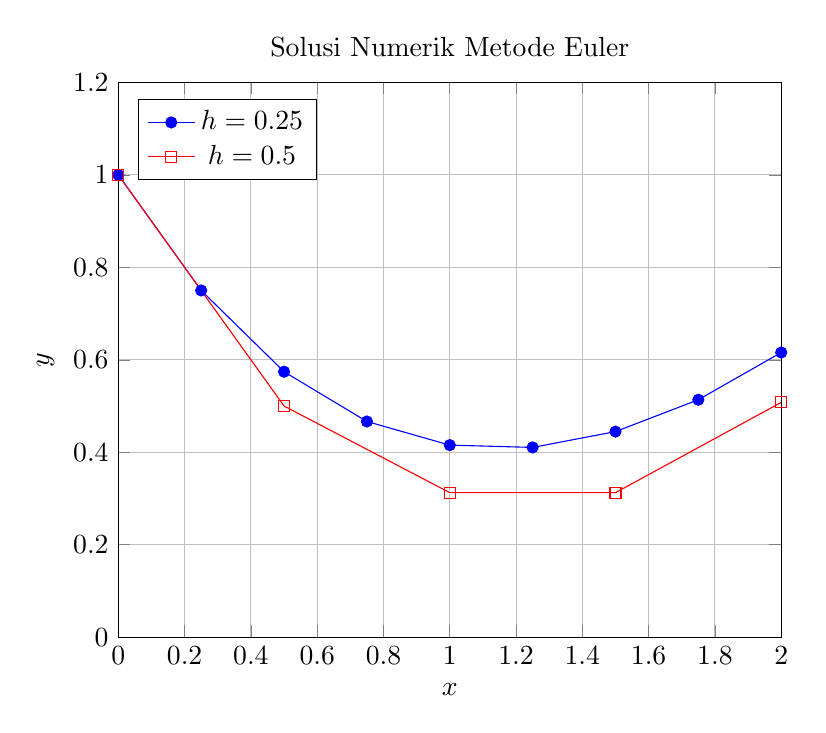
\begin{tikzpicture}
    \begin{axis}[
        title={Solusi Numerik Metode Euler},
        xlabel={\( x \)},
        ylabel={\( y \)},
        xmin=0, xmax=2,
        ymin=0, ymax=1.2,
        legend pos=north west,
        grid=both
    ]
    \addplot[blue, mark=*] coordinates {
        (0.00, 1.0000)
        (0.25, 0.7500)
        (0.50, 0.5742)
        (0.75, 0.4665)
        (1.00, 0.4154)
        (1.25, 0.4104)
        (1.50, 0.4446)
        (1.75, 0.5136)
        (2.00, 0.6158)
    };
    \addlegendentry{\( h = 0.25 \)}

    \addplot[red, mark=square] coordinates {
        (0.0, 1.0000)
        (0.5, 0.5000)
        (1.0, 0.3125)
        (1.5, 0.3125)
        (2.0, 0.5078)
    };
    \addlegendentry{\( h = 0.5 \)}
    \end{axis}
    \end{tikzpicture}
    \end{center}

    \textbf{Kesimpulan}
    \begin{itemize}
        \item \( h = 0.25 \) memberikan solusi yang lebih halus dan akurat dibandingkan \( h = 0.5 \).
        \item Grafik menunjukkan bahwa nilai \( y \) turun hingga \( x \approx 1.25 \), lalu naik kembali.
    \end{itemize}

    \item Selesaikan permasalahan di atas menggunakan metode Heun dengan (a) $h = \num{0,25}$; dan (b) $h = \num{0,5}$. Gambarkan pula grafik solusi yang telah anda buat. \\
    \penyelesaian 
    Rumus Metode Heun adalah:
    \[
    y_{i+1} = y_i + \frac{h}{2} \left[f(x_i, y_i) + f(x_{i+1}, \tilde{y}_{i+1})\right]
    \]
    dengan:
    \[
    \tilde{y}_{i+1} = y_i + h f(x_i, y_i)
    \]

    \begin{itemize}

    \item {\bf Langkah (a): \(h = 0{,}25\)}  
        \[
        \begin{array}{@{}c@{\;}c@{\;}c@{\;}c@{\;}c@{}}
        \toprule
        i & x_i  & y_i        & \tilde y_{i+1} & y_{i+1}     \\
        \midrule
        0 & 0.00 & 1.000000   & 1.000000       & 0.78710938  \\
        1 & 0.25 & 0.78710938 & 0.72119141     & 0.63837337  \\
        2 & 0.50 & 0.63837337 & 0.54572724     & 0.55016065  \\
        3 & 0.75 & 0.55016065 & 0.44013788     & 0.52007374  \\
        4 & 1.00 & 0.52007374 & 0.52007374     & 0.55664142  \\
        5 & 1.25 & 0.55664142 & 0.55664142     & 0.69498638  \\
        6 & 1.50 & 0.69498638 & 0.86872847     & 1.03874674  \\
        7 & 1.75 & 1.03874674 & 1.89693008     & 1.89693008  \\
        \midrule
        8 & 2.00 & 1.89693008 & —              & —           \\
        \bottomrule
        \end{array}
        \]
        Jadi \(y(2)\approx1.89693\).

    \item {\bf Langkah (b): \(h = 0{,}5\)}  
        \[
        \begin{array}{@{}c@{\;}c@{\;}c@{\;}c@{\;}c@{}}
        \toprule
        i & x_i  & y_i        & \tilde y_{i+1} & y_{i+1}     \\
        \midrule
        0 & 0.0  & 1.000000   & 1.000000       & 0.65625000  \\
        1 & 0.5  & 0.65625000 & 0.49218750     & 0.53320312  \\
        2 & 1.0  & 0.53320312 & 0.00000000     & 0.69982910  \\
        3 & 1.5  & 0.69982910 & 1.21206548     & 1.77144241  \\
        \midrule
        4 & 2.0  & 1.77144241 & —              & —           \\
        \bottomrule
        \end{array}
        \]
        Jadi \(y(2)\approx1.77144\).

    \end{itemize}

    \bigskip
    \noindent Berikut grafik solusi \(y(x)\) untuk kedua ukuran langkah:

    \begin{center}
    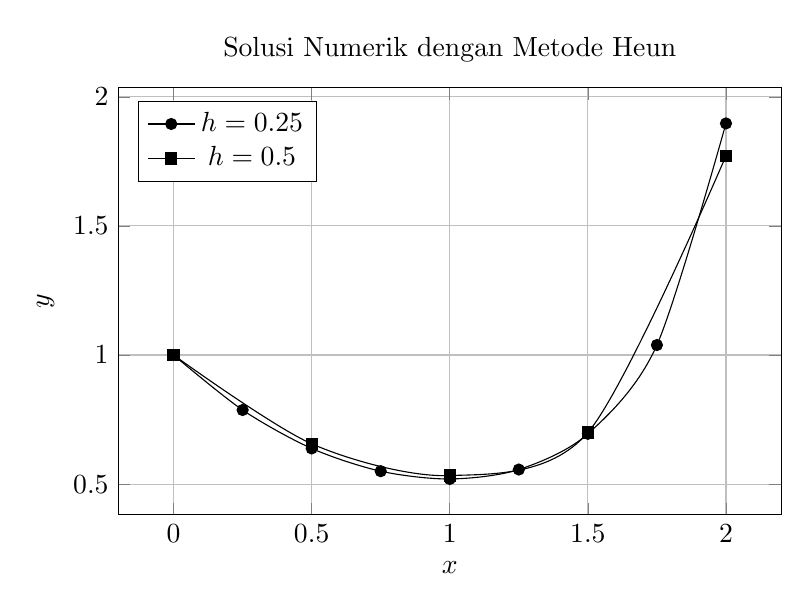
\begin{tikzpicture}
    \begin{axis}[
        width=10cm, height=7cm,
        xlabel={$x$}, ylabel={$y$},
        title={Solusi Numerik dengan Metode Heun},
        legend pos= north west,
        grid=major,
    ]
        \addplot[mark=*, smooth] coordinates {
        (0.00,1.000000) (0.25,0.787109) (0.50,0.638373) (0.75,0.550161)
        (1.00,0.520074) (1.25,0.556641) (1.50,0.694986) (1.75,1.038747)
        (2.00,1.896930)
        };
        \addlegendentry{$h=0.25$}

        \addplot[mark=square*, smooth] coordinates {
        (0.00,1.000000) (0.50,0.656250) (1.00,0.533203) (1.50,0.699829)
        (2.00,1.771442)
        };
        \addlegendentry{$h=0.5$}
    \end{axis}
    \end{tikzpicture}
    \end{center}

    \item Selesaikan permasalahan di atas menggunakan metode RK-2 Ralston dengan (a) $h = \num{0,25}$; dan (b) $h = \num{0,5}$. Gambarkan pula grafik solusi yang telah anda buat. \\
    \penyelesaian 
    Bentuk persamaan RK-2 metode Ralston:
    \begin{equation*}
        y_{i+1} = y_i + (\frac{1}{3}k_1 + \frac{2}{3}k_2)h
    \end{equation*}
    dengan
    \begin{flalign*}
        & k_1 = f(x_i, y_i) && \\
        & k_2 = f\left (x_i + \frac{3}{4}h, y_i + \frac{3}{4}k_1h \right ) &&
    \end{flalign*}

    \begin{enumerate}
        \item $h = \num{0,25}$ \\
        Asumsikan $(x_0, y_0) = (0, 1)$, sehingga
        \begin{flalign*}
            & k_1 = f(0, 1) = (1)(0)^2 - (1) = -1 && \\
            & k_2 = f\left ((0) + \frac{3}{4}(\num{0,25}), (1) + \frac{3}{4}(-1)(\num{0,25}) \right ) = f(\num{0,1875}, \num{0,8125}) \approx \num{-0,7839}&&
        \end{flalign*}
        dan diperoleh nilai $y_1$:
        \begin{flalign*}
            & y_{1} = (1) + \left (\frac{1}{3}(-1) + \frac{2}{3}(\num{-0,7839})\right )(\num{0,25}) \approx \num{0,7860}&&
        \end{flalign*}
        Selanjutnya, hasil iterasi metode RK-2 Ralston hingga $x = 2$ disajikan dalam tabel berikut. \\
        \begin{tabular}{|c|c|c|c|c|c|}
            \hline
            $i$ & $x_i$ & $y_i$ & $k_1$ & $k_2$ & $y_{i+1}$ \\
            \hline
            0 & \num{0} & \num{1} & \num{-1} & \num{-0,7839} & \num{0,7860} \\
            1 & \num{0,25} & \num{0,7860} & \num{-0,7369} & \num{-0,5238} & \num{0,6373} \\
            2 & \num{0,50} & \num{0,6373} & \num{-0,4780} & \num{-0,2888} & \num{0,5493} \\
            3 & \num{0,75} & \num{0,5493} & \num{-0,2403} & \num{-0,0611} & \num{0,5191} \\
            4 & \num{1} & \num{0,5191} & \num{0} & \num{0,2129} & \num{0,5546} \\
            5 & \num{1,25} & \num{0,5546} & \num{0,3120} & \num{0,6538} & \num{0,6896} \\
            6 & \num{1,50} & \num{0,6896} & \num{0,8620} & \num{1,5727} & \num{1,0235} \\
            7 & \num{1,75} & \num{1,0235} & \num{2,1110} & \num{3,9088} & \num{1,8509} \\
            \hline
        \end{tabular} \\     

        \item $h = \num{0,5}$ \\
        Dengan asumsi $(x_0, y_0) = (0, 1)$, berikut tabel hasil iterasi metode RK-2 Ralston hingga $x = 2$. \\
        \begin{tabular}{|c|c|c|c|c|c|}
            \hline
            $i$ & $x_i$ & $y_i$ & $k_1$ & $k_2$ & $y_{i+1}$ \\
            \hline
            0 & \num{0} & \num{1,0000} & \num{-1} & \num{-0,5371} & \num{0,6543} \\
            1 & \num{0,50} & \num{0,6543} & \num{-0,4907} & \num{-0,1102} & \num{0,5358} \\
            2 & \num{1} & \num{0,5358} & \num{0} & \num{0,4772} & \num{0,6948} \\
            3 & \num{1,50} & \num{0,6948} & \num{0,8685} & \num{2,5673} & \num{1,6953} \\
            \hline
        \end{tabular} \\     
    \end{enumerate}
    Berdasarkan tabel-tabel di atas, berikut grafik solusi permasalahan di atas menggunakan metode RK-2 Ralston. \\

    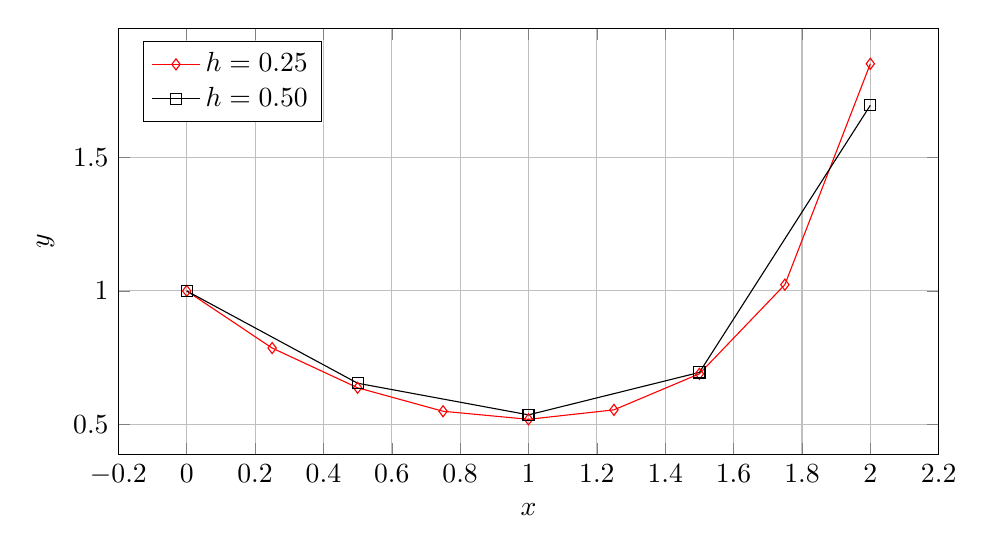
\begin{tikzpicture}
        \begin{axis}[
            xlabel=$x$, ylabel=$y$,
            grid=both,
            width=12cm, height=7cm,
            legend pos=north west
        ]
    
        \addplot[
            mark=diamond, 
            mark size=2pt, 
            color=red,
        ] coordinates {
            (0,1)
            (0.25,0.7860)
            (0.50,0.6373)
            (0.75,0.5493)
            (1.0,0.5191)
            (1.25,0.5546)
            (1.50,0.6896)
            (1.75,1.0235)
            (2.0,1.8509)
        };
        \addlegendentry{$h = 0.25$}
        
        % Optionally connect points with a line
        \addplot[
            mark=square, 
            mark size=2pt, 
            color=black,
        ] coordinates {
            (0,1)
            (0.50,0.6543)
            (1.0,0.5358)
            (1.50,0.6948)
            (2.0,1.6953)
        };
        \addlegendentry{$h = 0.50$}

        \end{axis}
    \end{tikzpicture}
\end{enumerate}

\end{document}